\documentclass[20pt,,margin=1in,innermargin=-4.5in,blockverticalspace=-0.25in]{tikzposter}
\geometry{paperwidth=43in,paperheight=32.5in}
\usepackage[utf8]{inputenc}
\usepackage{amsmath}
\usepackage{amsfonts}
\usepackage{amsthm}
\usepackage{amssymb}
\usepackage{mathrsfs}
\usepackage{graphicx}
\usepackage{adjustbox}
\usepackage{enumitem}
\usepackage{wrapfig}
\usepackage{SUtheme}
\usepackage{comment}
\usepackage{mwe} % for placeholder images

% set theme parameters
\tikzposterlatexaffectionproofoff
\usetheme{SUTheme}
\usecolorstyle{SUStyle}
\usetitlestyle{Filled}

\usepackage[scaled]{helvet}
\renewcommand\familydefault{\sfdefault} 
\usepackage[T1]{fontenc}


\title{An Overdetermined Symmetry Problem}
\author{Ethan Martirosyan, Yingpeng HE Mentor: Jihye Lee}
\institute{University of California Santa Barbara}
\titlegraphic{
\includegraphics[width=0.06\textwidth]{logo.png}}

% begin document
\begin{document}
\maketitle
\centering

\begin{columns}
    \column{0.32}
    \block{Introduction}{
                  Let us consider the following problem. Let $\Omega \subseteq \mathbb{R}^n$ be a domain that is bounded, open, and connected. Furthermore, suppose that the boundary $\partial{\Omega}$ is smooth. Let $u: \Omega \rightarrow \mathbb{R}$ be a $C^2$ function that satisfies the following conditions: $\Delta u = -1$ in $\Omega$. and $u=0$ and $\frac{\partial{u}}{\partial{n}} = c$ on $\partial{\Omega}$ for some constant $c$. Then, $\Omega$ must be a ball. Furthermore, we know that $u(x) = (b^2-r^2)/2n$, where $b$ is the ball's radius and $r$ is the distance to its center. 
    }
    \block{First Proof}{
     The first proof we present is from Professor James Serrin [3].
    This proof utilizes the moving plane method. Let $T_0$ be a $n-1$ dimensional hyperplane in $\mathbb{R}^n$ that does not intersect the domain $\Omega$. We begin to move this plane in a direction normal to itself until it intersects $\Omega$. When this occurs, the new plane $T$ splits $\Omega$ into two parts. The part of $\Omega$ that lies on the same side of $T$ as our initial plane $T_0$ is denoted by $\Sigma(T)$. We reflect $\Sigma(T)$ in $T$ to obtain $\Sigma^\prime := \Sigma^\prime(T)$. As $T$ moves through $\Omega$, $\Sigma^\prime$ will remain in $\Omega$ until the set $\Sigma^\prime$ meets $\Omega$ at a point $P$ or $T$ becomes orthogonal to $\Omega$ at some point $Q$. When either of these occurs, we stop moving the plane $T$, and we denote the resulting plane by $T^\prime$. We claim that $\Omega$ is symmetric about $T^\prime$. Showing this would prove the theorem. To see how, we recall that the plane $T_0$ was chosen arbitrarily. If $\Omega$ is symmetric about $T^\prime$, then $\Omega$ is symmetric in all possible directions. Since $\Omega$ is simply connected and has this strong symmetry property, it must be a ball.
      \begin{align*} 
            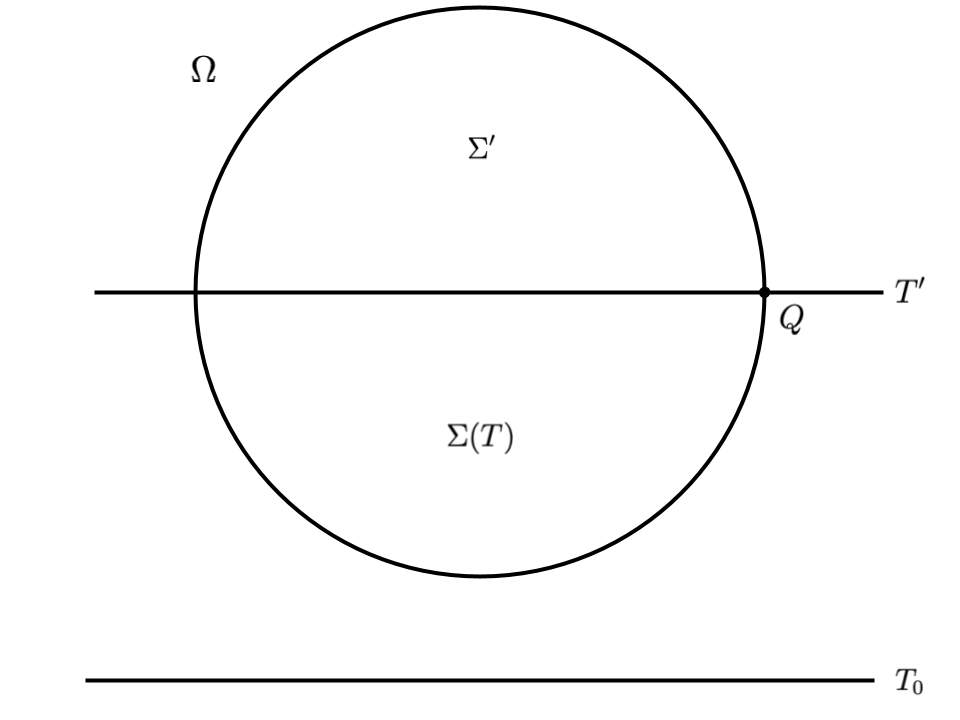
\includegraphics[width=.29\textwidth]{Image1}
         \end{align*}

    To prove this, we introduce the function $v: \Sigma^\prime \rightarrow \mathbb{R}$ defined by $v(x) = u(x^\prime)$ for $x \in \Sigma^\prime$, where $x^\prime$ is the reflection of $x$ across $T^\prime$. By the maximum principle, we deduce that $u - v > 0$ or $u-v = 0$ in $\Sigma^\prime$. Suppose that $u-v > 0$.  If $\Sigma^\prime$ is internally tangent to $\Omega$ at some point $P$, then we may appeal to the boundary point maximum principle to deduce that $\frac{\partial}{\partial{n}}(u-v) > 0$ at $P$ [1]. However, we know that $\partial{u}/\partial{n} = \partial{v}/\partial{n} = c$. If $T^\prime$ is orthogonal to the boundary of $\Omega$ at some point $Q$, then we show that $u$ and $v$ have the same first and second derivatives at $Q$. Using a modified version of the boundary point maximum principle, we can also show that $\frac{\partial}{\partial{s}} (u-v) > 0 \text{ or } \frac{\partial^2}{\partial^2{s}}(u-v) > 0$ for any direction $s$ that enters $\Sigma^\prime$ non-tangentially at $Q$. However, this directly contradicts the fact that $u$ and $v$ have the same first and second derivatives at $Q$. We may thus conclude that $\Omega$ is symmetric about $T^\prime$.
}


    \column{0.36}
    \block{Second Proof}{
        The second proof we present is from Weinberger [2]. To start, we first compute
\[
\Delta\bigg(r \frac{\partial{u}}{\partial{r}}\bigg) = r \frac{\partial}{\partial{r}} (\Delta u) + 2\Delta = -2
\] where $r$ is the distance to the origin. Using this and the fact that $\Delta u = -1$, we obtain
\[
\int_\Omega \bigg[ 2u - r\frac{\partial{u}}{\partial{r}}\bigg] dx = \int_\Omega \bigg[ -u \Delta \bigg(r \frac{\partial{u}}{\partial{r}} \bigg) + r \frac{\partial{u}}{\partial{r}} \Delta u \bigg] dx
\]
    Using Green's identity yields
\[
\int_\Omega \bigg[ -u \Delta \bigg(r \frac{\partial{u}}{\partial{r}} \bigg) + r \frac{\partial{u}}{\partial{r}} \Delta u \bigg] dx = \int_{\partial{\Omega}} \bigg[ - u \frac{\partial}{\partial{n}}\bigg(r\frac{\partial{u}}{\partial{r}}\bigg)+ r \frac{\partial{u}}{\partial{r}}\frac{\partial{u}}{\partial{n}}\bigg] dS
\] By assumption, we have $u = 0$ on the boundary of $\Omega$. Thus, we find that
\[
\int_{\partial{\Omega}} \bigg[ - u \frac{\partial}{\partial{n}}\bigg(r\frac{\partial{u}}{\partial{r}}\bigg)+ r \frac{\partial{u}}{\partial{r}}\frac{\partial{u}}{\partial{n}}\bigg] dS =  \int_{\partial{\Omega}} r \frac{\partial{r}}{\partial{n}} \bigg(\frac{\partial{u}}{\partial{n}}\bigg)^2 dS
\] By assumption, we know that $\partial{u}/\partial{n} = c$ on the boundary of $\Omega$. Thus, we find that
\[
\int_{\partial{\Omega}} r \frac{\partial{r}}{\partial{n}} \bigg(\frac{\partial{u}}{\partial{n}}\bigg)^2 dS = c^2 \int_{\partial{\Omega}} r\frac{\partial{r}}{\partial{n}} dS
\] Appealing to the Divergence Theorem and using the fact that $\Delta \frac{1}{2}r^2 = r \Delta r$, we obtain
\[
c^2 \int_{\partial{\Omega}} r\frac{\partial{r}}{\partial{n}} dS = c^2 \int_{\Omega} \Delta\bigg(\frac{1}{2}r^2\bigg) dx = c^2 n \int_{\Omega} dx =  nc^2 V
\] Green's theorem also implies
\[
\int_{\Omega} r \frac{\partial{u}}{\partial{r}} dx = -n \int_{\Omega} u dx
\] so that substitution yields
\[
(n+2) \int_\Omega u d x = nc^2V
\] However, we also note that
\[
1 = (\Delta u)^2 \leq n \sum_{i=1}^n u_{ii}^2 \leq n \sum_{i,j} u_{ij}^2
\] by the Cauchy-Schwarz inequality. From this, we deduce that
\[
\Delta\bigg( \vert \nabla u\vert^2 + \frac{2}{n}u\bigg) = 2\sum_{i,j} u_{ij}^2 - \frac{2}{n} \geq 0
\] Using this and the fact that $\vert \nabla u \vert^2 + (2/n)u = c^2$ on $\partial{\Omega}$, we may appeal to the maximum principle to deduce that $\vert \nabla u \vert + (2/n)u < c^2$ in $\Omega$ or $\vert \nabla u \vert + (2/n)u = c^2$ in $\Omega$. If the former inequality held, then we could integrate over $\Omega$ to deduce that
\[
(n+2)\int_\Omega u dx < nc^2V
\] This contradiction informs us that $\vert \nabla u \vert^2 + (2/n)u = c^2$ in $\Omega$ so that
\[
1 = n \sum_{i=1}^n u_{ii}^2 = \sum_{i,j} u_{ij}^2
\] which implies that $u_{ij} = -\delta_{ij}/n$. Solving the corresponding partial differential equations yields
\[
u = \frac{1}{2n}(B - r^2)
\] where $B$ is a constant. Since $u = 0$ on $\partial{\Omega}$, $B$ is positive and $\Omega$ is a ball of radius $B^{1/2}$.

    }

    \column{0.32}
    \block{Applications}{
       This theorem is significant because it allows us to determine the shape of $\Omega$ from properties of $u$. It also has many applications in physics. For example, we may consider an incompressible viscous fluid moving through a straight pipe of cross sectional form $\Omega$. If we fix a rectangular coordinate system with the $z$-axis directed along the pipe, then the velocity $u$ depends only on $x$ and $y$, and it satisfies the differential equation $\Delta u = -A$ for some constant $A$. Furthermore, because the fluid is viscous, we know that $u = 0$ on $\partial{\Omega}$; that is, there is no movement on the boundary of the pipe. Finally, we note that $\mu\partial{u}/\partial{n}$ is the tangential stress on the pipe wall, where $\mu$ is the viscosity constant. If the tangential stress is constant, then we may apply the above theorem to conclude that $\Omega$ is a circular cross section. 
    }
    \block{Generalizations}{
    There is an interesting extension of this theorem from Wolfgang Reichel [4]. Let $\Omega_1$ be a bounded domain with smooth boundary, and suppose that $\Omega = \mathbb{R}^n \setminus \overline{\Omega}_1$ is connected. Let $u$ be a twice continuously differentiable function on $\overline{\Omega}$ such that $\Delta u + f(u, \vert \nabla u \vert) = 0$ in $\overline{\Omega}$, $0 \leq u < a$ in $\Omega$, $u = a$ and $\partial{u}/\partial{n} = c \leq 0$ on $\partial{\Omega_1}$, and $u = \nabla u = 0$ at $\infty$. Furthermore, suppose that $f(p,q)$ is Lipschitz continuous in $p$ and $q$ and decreasing in $p$. Then, we may conclude that $\Omega_1$ is a ball and that $u$ is radially symmetric and decreasing in $r$. This can be proved by the moving plane method.
    \begin{align*} 
            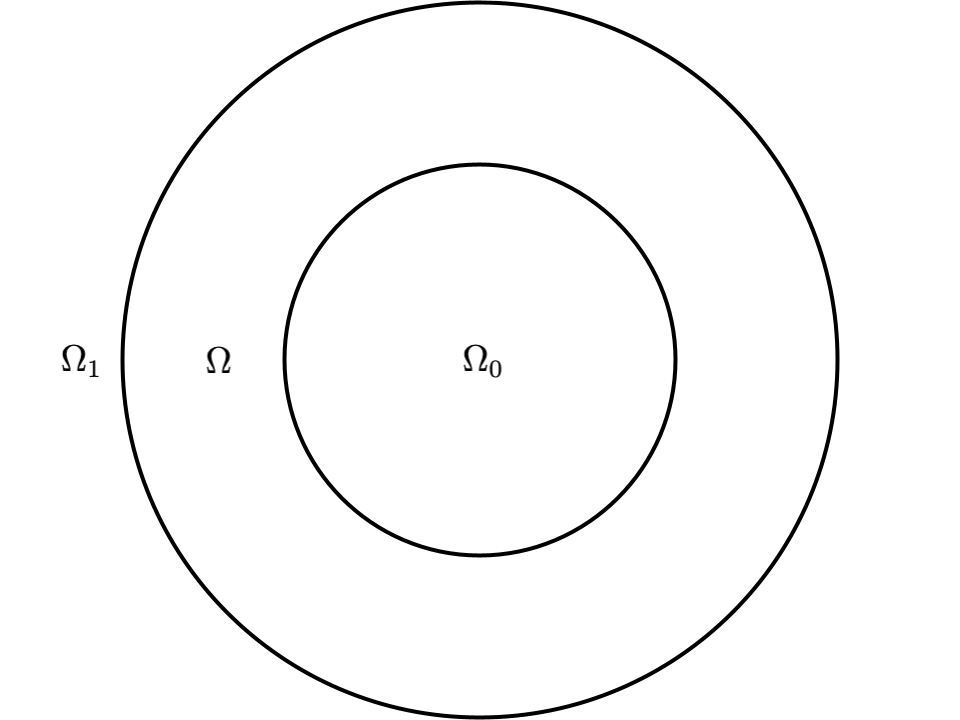
\includegraphics[width=.25\textwidth]{Image2}
         \end{align*}
    }    
    \block{Acknowledgements}{
    	We would like to thank Jihye Lee for mentoring us. Furthermore, we express gratitude to the 2024 UCSB Directed Reading Program for giving us this opportunity.
    }
    
    \block{References}{
    	\footnotesize
    	
	[1] Hans Weingberger. Maximum Principles in Differential Equations. 1984.
	
	[2] Hans Weingberger. Remark on the Preceding Paper of Serrin. \emph{Arch. Rational Mech. Anal.} 1971.
		
	[3] James Serrin. A Symmetry Problem in Potential Theory. \emph{Arch. Rational Mech. Anal.} 1971.
		
	[4] Wolfgang Reichel. Radial Symmetry for Elliptic Boundary-Value Problems on Exterior Domains. \emph{Arch. Rational Mech. Anal.}. 1997.
	
	
    }
\end{columns}
\end{document}
